\documentclass{article}
\usepackage{geometry}
\usepackage{xcolor}
\usepackage{tikz} 
\usetikzlibrary{arrows, positioning, calc, shadows, fadings}


\geometry{
	a4paper,
	total={170mm,257mm},
	left=20mm,
	top=20mm,
}


\begin{document}
	
	
	\section*{CPU Normal Execution (Fetch and Execute Cycle)}
	
	\begin{center}
		
	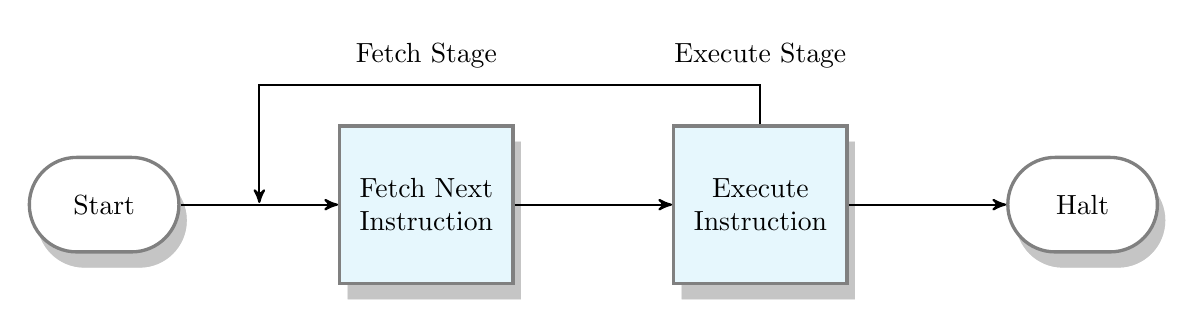
\begin{tikzpicture}[
		node distance = 2cm,
		inner sep=2mm, 
		shorten <=0pt, 
		>=stealth', 
		thick,
		roundrectangle/.style={
				rectangle,
				minimum width = 15mm,
				text width = 15mm,
				align=center,
				minimum height = 12mm,
				rounded corners=6mm,
				very thick,
				draw=black!50,		
				fill=white,		
				drop shadow={
					top color=black!20,
					bottom color=black!20,
					shadow xshift=1mm,
					shadow yshift=-2mm
				}
			},		
		cornerrectangle/.style={
				rectangle, 
				minimum size = 20mm,  
				text width=18mm,
				align=center,
				very thick,
				draw=black!50,			
				fill=cyan!10,
				drop shadow={
					top color=black!20,
					bottom color=black!20,
					shadow xshift=1mm,
					shadow yshift=-2mm
				}
			},
		] 
		 
		\node[roundrectangle] (start) {Start};
		
		\node[cornerrectangle, right= of start] (fetch) {Fetch Next Instruction};				
		
		\node[cornerrectangle, right= of fetch] (execute) {Execute Instruction};
		
		\node[roundrectangle, right= of execute] (halt) {Halt};
		
		\draw[->] (start) -- (fetch);
		
		\draw[->] (fetch) -- (execute);
		
		\draw[->] (execute) -- (halt);
		
		\draw[->] (execute.north) -- ++(0, 0.5) -- ($(fetch.north west) + (-1,0.5) $) -- ++(0,-1.5);
		
		\node[above= of execute, yshift=-1.5cm] {Execute Stage};
		
		\node[above= of fetch, yshift=-1.5cm] {Fetch Stage};
		
	\end{tikzpicture}
			
	\end{center}

\end{document}